%*****************************************
\chapter{Implementation}
\label{ch:implementation}
%*****************************************

\hint{This chapter should describe the details of the implementation addressing the following questions: \\ \\
1. What are the design decisions made? \\
2. What is the environment the approach is developed in? \\
3. How are components mapped to classes of the source code? \\
4. How do the components interact with each other?  \\
5. What are limitations of the implementation? \\ \\
The section should have a length of about five pages.}
\section{Design Decisions}
\begin{itemize}
	\item tensorflow 2.0
	\item scikit-learn
	\item pickle
\end{itemize} 

\section{Architecture}
\begin{figure}[H]
	\centering
	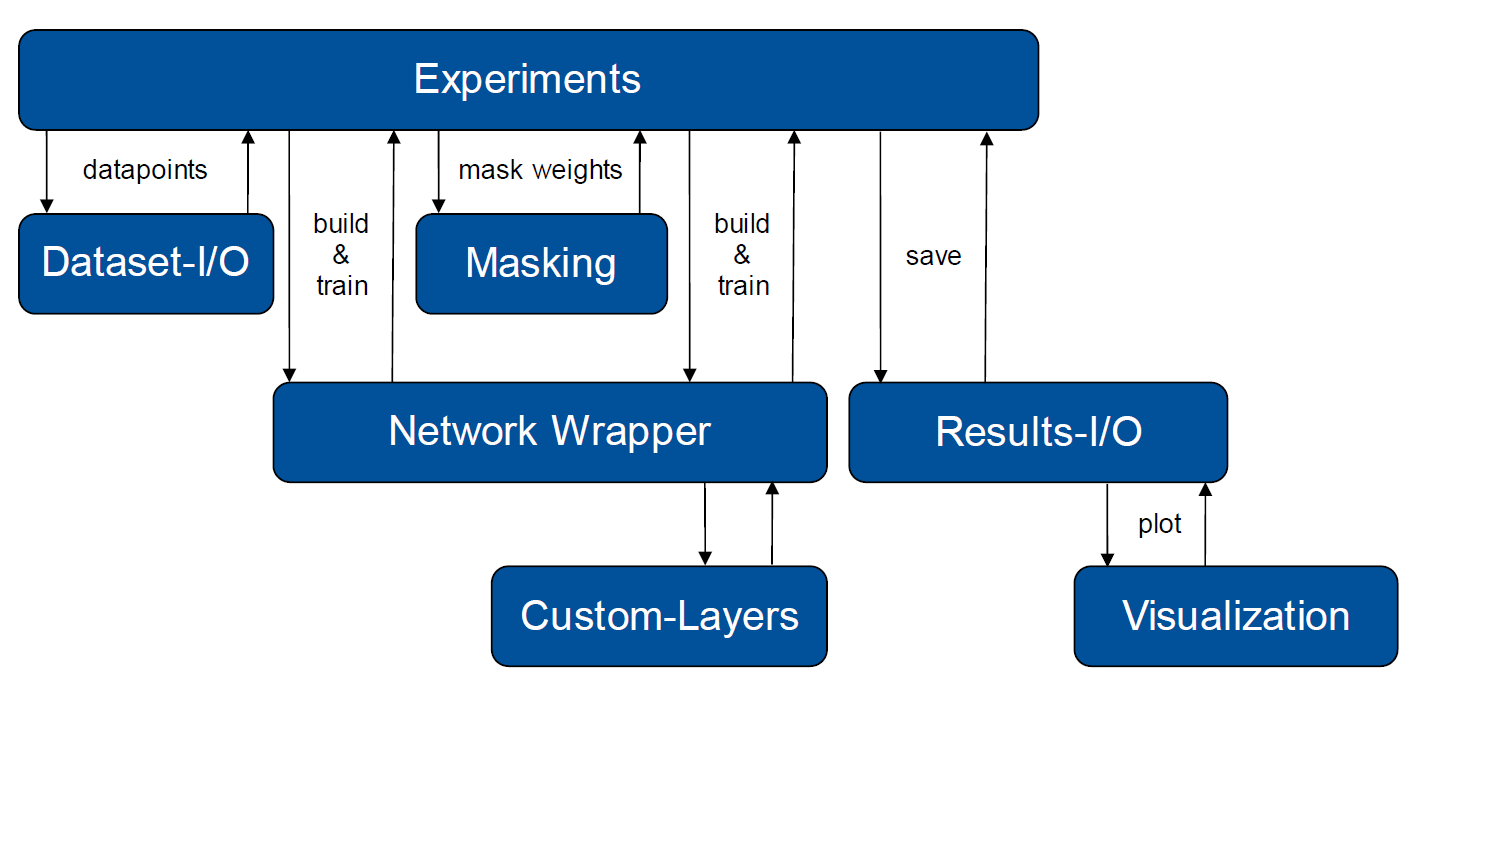
\includegraphics[width=450px]{gfx/structure.png}
	\caption{project architecture}
	\label{fig:Architecture}
\end{figure}

\section{Interaction of Components}
\begin{figure}[H]
	\centering
	\includegraphics[width=450px]{gfx/structure2.png}
	\caption{project architecture}
	\label{fig:Interaction}
\end{figure}


\section{Summary}